\documentclass[10pt,a4paper]{article}

\usepackage[utf8]{inputenc}
\usepackage[polish]{babel}
\usepackage[T1]{fontenc}
\usepackage{amsmath}
\usepackage{amsfonts}
\usepackage{anysize}
\usepackage{fancyhdr}
\usepackage{setspace}
\usepackage{url}
\usepackage{graphicx}
\usepackage{minibox}
\usepackage{paralist}
\usepackage{framed}
\usepackage{listings}
\usepackage{color}
\usepackage{float}
\usepackage{array}
\usepackage{tgpagella}
\usepackage[scaled]{helvet}
\usepackage{titlesec}
\usepackage{graphicx}


\renewcommand\thesection{\arabic{section}.}
\renewcommand\thesubsection{\arabic{section}.\arabic{subsection}.}
\renewcommand\thesubsubsection{\arabic{section}.\arabic{subsection}.\arabic{subsubsection}.}
\renewcommand{\footrulewidth}{0.4pt}% Default \footrulewidth is 0pt

\marginsize{2cm}{2cm}{2cm}{2cm}
\setlength{\parindent}{0pt}

\title{Techniki Internetowe\\
       \textbf{Projekt}}

\date{semestr 14L}

\author{Patrycja Dybka\\
		Bartosz Frączak\\
		Damian Rakowski\\
		Wiktor Ślęczka}

\pagestyle{fancy}

\definecolor{dkgreen}{rgb}{0,0.6,0}
\definecolor{gray}{rgb}{0.5,0.5,0.5}
\definecolor{mauve}{rgb}{0.58,0,0.82}

\lstset{frame=tb,
  language=Bash,
  aboveskip=3mm,
  belowskip=3mm,
  showstringspaces=false,
  xleftmargin=15pt,
  xrightmargin=15pt,
  frame=none,
  columns=flexible,
  basicstyle={\small\ttfamily},
  numbers=none,
  numberstyle=\tiny\color{gray},
  keywordstyle=\color{blue},
  commentstyle=\color{dkgreen},
  stringstyle=\color{mauve},
  breaklines=true,
  breakatwhitespace=true
  tabsize=3
}


\begin{document}

\maketitle
\newpage

\tableofcontents
\newpage

\section{Treść zadania}
Zadanie polega na napisaniu prostego programu P2P (Peer-to-Peer) umożliwiającego rozproszone przechowywanie zasobów.
\section{Interpretacja zadania}
Głównym elementem naszego projektu jest działający w tle proces,
nazywany serwerem\footnote{Dla rozróżnienia z klientem, który jest
używany do bezpośredniej komunikacji z użytkownikiem}.
Zarządza on w naszym programie zasobami oraz zapewnia komunikację z innymi
programami w sieci. Gdy plik zostanie umieszczony w węźle, broadcastuje on
zdarzenie. Wtedy każdy odbiorca jest zobowiązany odpowiedzieć na nie,
natomiast nadawca pierwszej otrzymanej odpowiedzi stanie się
nowym właścicielem nowo dodanego pliku.
Plik na węźle, na którym został umieszczony zostaje kopią,
natomiast plik zostaje skopiowany do losowego węzła, który staje się
jego właścicielem.\\
\\
Synchronizacja posiadanych zasobów jest przeprowadzana kompletnie, synchronizowana jest cała lista plików, nie tylko to, co się zmieniło, i zawsze, gdy:
\begin{itemize}
\item Zmieni się stan przechowywanych plików.
\item Dołączy/zostanie uruchomiony nowy węzeł.
\item Na wyraźne życzenie użytkownika.
\end{itemize}

Pliki przesyłane są binarnie, a pozostałe informacje przekazywane są za pomocą formatu $JSON$.\\
\\Uruchomiony proces serwera cyklicznie sprawdza polecenia od programu klienckiego używanego do komunikacji z użytkownikiem. W przypadku gdy użytkownik rozkaże pobranie pliku, żądanie jest rozgłaszane pomiędzy węzły. Jeśli węzeł posiada poszukiwany plik, zgłasza się do odpowiedniego węzła. Następnie plik jest pobierany w równej częśći z każdego węzła, który go posiada. Problem, gdy plik o tej samej nazwie zostanie dodany na dwóch różnych komputerach nie występuje, gdyż do nazwy dodawana jest sól, generowana na podstawie adresu węzła posiadającego oryginał.\\

Wszystkie pliki przechowywane są we wspólnym katalogu, pod swoją pełną nazwą.



\section{Opis funkcjonalny}
Program z punktu użytkownika będzie udostępniał następujące polecenia:\\
\begin{itemize}
\item start$[nazwa]$\\
Uruchomienie serwera z nazwa jako nazwa hosta. Jeśli nazwa nie jest podana, jest generowana automatycznie.
\item restart$[nazwa]$\\
Ponowne uruchomienie serwera z nazwa jako nazwa hosta. Jeśli nazwa nie jest podana, jest generowana automatycznie.

\item stop\\
Zatrzymanie działania serwera.

\item add sciezka/do/pliku$[nazwa$ $pliku]$\\
Dodanie pliku do zasobów serwera. Jeśli podana jest nazwa, plik zostanie dodany pod tą nazwą. W przeciwnym wypadku, plik zostanie dodany pod swoją nazwą.

\item get nazwa pliku $[sciezka/do/pliku]$\\
Pobranie pliku z innych węzłów, jeśli plik nie został dodany do lokalnego,
oraz skopiowanie go w podane miejsce. Jeśli podana zostanie ścieżka,
plik zostanie zapisany na podanej ścieżce. W przeciwnym przypadku,
plik zostanie zapisany w aktualnym katalogu, pod nazwą występującą w aplikacji.
\item download nazwa pliku$[nazwa$ $hosta]$\\
Pobranie pliku z innych węzłów w celu udostępniania. Nie kopiuje pliku poza wewnętrzne dane programu. Jeśli podana jest nazwa hosta, ściagany plik jest tylko od żadanego węzła.

\item rescan\\
Pobranie aktualnej listy plików z sieci, oraz uaktualnienie listy węzłów.

\item show-list\\
Wyświetlenie listy plików w sieci.
\item remove $nazwa$$pliku$\\
Usunięcie pliku.
\end{itemize}
\section{Protokół}
Protokół bazowany jest na formacie JSON - JavaScript Object Notation.
Wszystkie podane tutaj komunikaty wysyłane są poprzez UDP. Jedyny moment,
kiedy używane jest TCP/IP w naszym projekcie to wymiana plików w trybie
binarnym.

\begin{itemize}
\item Podczasz uruchomienia programu na jednym z komputerów, rozgłasza on swoją obecność (pakiet: "Hello"), na co pozostałe peery odpowiadają analogicznym zgłoszeniem (tylko w sytuacji, gdy nie wiedziały o tym, który aktualnie się identyfikuje, w celu zapobiegnięcia zapętleniu). Jeżeli w odpowiedzi program dostanie “Hello’ od innego uzytkownika z taka nazwa, wyświetli on komunikat dla użytkownika o niedostępności nazwy.
\renewcommand{\labelitemii}{$\circ$}
\begin{itemize}
\item \{“type”: “Hello”, “name”: “LosowyHost”\}
\end{itemize}
\item Dowolny z peerów może zainicjować rozgłaszanie zasobów, poprzez pakiet "GiveFilelist", wtedy każdy odbiorca tego pakietu jest zobowiązany odpowiedzieć broadcastem pakietem "IHave", zawierający listę plików, oraz informację o tym, czy jest ich właścicielem. Każdy posiadający kopię powinien przy otrzymaniu isOwner przedłuzyć datę ważności.
\begin{itemize}
\item \{“type”: “GiveFilelist”, “name”: “jakishost”\}
\item \{“type”: “IHave”, “name”: “jakishost”,“files”: [\{“file”: “pliktestowy”,
\\“md5”: “1de806ceee9f3172d154275a90fb148a”,“isOwner”: true, “expires”: 1398717645\},
\\\{“name”: “pliknietestowy”, “md5”: “20dc258bb9b0b3ce53a32d1df7b1b50f”, “isOwner”: false,
\\“expires”: 1398717645\}]\}
\end{itemize}
\item Dowolny z peerów może pobrać plik z innego peera. W tym celu wysyła pakiet typu ''GiveMe'' z informacją o tym, jaki plik chce uzyskać oraz portem, na którym nasłuchuje. Hosty posiadające ten plik, zobowiązane są do nawiązania połączenia na ten port przy pomocy TCP/IP. Po połączeniu się, za posiadacz pliku binarnie podaje identyfikator pliku, jego hash i rozmiar, poszukiwacz odpowiada, czy nadal chce ten plik i w jakim stopniu albo zamyka połączenie, a następnie zawartość pliku jest wysyłana przez posiadacza. Ostatnia część procesu może być powtarzana W przypadku, gdy nie było odpowiedzi, poszukiwacz ponawia zapytanie, a w przypadku ponownego błędu informuje użytkownika o błędzie i aktualizuje listę plików/hostów. Data wazności w przypadku oryginałów jest ustawiana na ''0''
\begin{itemize}
\item \{“type”: “GiveMe”, “name”: “jakishost”, “file”: “pliktestowy”,
\\“md5”: “20dc258bb9b0b3ce53a32d1df7b1b50f”, “original”: false\}
\item <TCP/IP>
\begin{itemize}
\renewcommand{\labelitemiii}{$\circ$}
\item Dowolny z peerów może zakomunikować dodanie nowego pliku
\\Wysylajacy:pliktestowy\textbackslash n20dc258bb9b0b3ce53a32d1df7b1b50f\textbackslash nwielkosc pliku\textbackslash r\textbackslash nexpirydate\textbackslash n
\item Odbierajacy: offset\textbackslash nwielkosckawalka\textbackslash n
\item Wysylajacy:jakiesdanebinarne
\item Odbierający offset2\textbackslash nwielkosckawalka2\textbackslash n
\item Wysylajacy: jakiesdanebinarne2
\item u poprzez wysłanie pakietu typu ''IGot'' z informacją o nazwie zasobu. Po wysłaniu takiej wiadomości, odczekuje on 30sekund, po czym jeżeli nie nastąpi sprzeciw w postaci pakietu ''Objection'' ze specyfikatorem zasobu, uznaje on, że udało się poprawne dodanie. Hosty, które nie zgłosiły sprzeciwu zgłaszają wiadomość typu ''GiveMe'', aby uzyskać plik z prawami oryginału. Host wybiera pierwszy, który do niego dotrze.
\end{itemize}
\end{itemize}
\item Dowolny z peerów może zakomunikować dodanie nowego pliku poprzez wysłanie pakietu typu ''IGot'' z informacją o nazwie zasobu. Po wysłaniu takiej wiadomości, odczekuje on 30 sekund, po czym jeżeli nie nastąpi sprzeciw w postaci pakietu "Objection" ze specyfikatorem zasobu, uznaje on, że udało się poprawne dodanie. Hosty, które nie zgłosiły sprzeciwu zgłaszają wiadomość typu ''GiveMe'', aby uzyskać plik z prawami oryginału. Host wybiera pierwszy, który do niego dotrze.
\begin{itemize}
\item \{“type”: “IGot”, “file”: “nowyplik”, “md5”:”20dc258bb9b0b3ce53a32d1df7b1b50f”\}
\item \{“type”: “Objection”, “file”: “nowyplik”, “md5”:”20dc258bb9b0b3ce53a32d1df7b1b50f”\}
\item \{“type”: “GiveMe”, “file”: “nowyplik”, “md5”: “20dc258bb9b0b3ce53a32d1df7b1b50f”, “original”: true\}
\end{itemize}
\item Dowolny z peerów posiadający oryginał może go unieważnić poprzez pakiet typu "Forget" i wiadomością o tym, jaki to zasób. Hosty posiadające kopię odpowiadają pakietem typu "IForgot" oraz oznaczają dany zasób jako nietransferowalny i po jakimś czasie usuwają
go. Czynność ta jest także dozwolona, gdy nie posiada się oryginału,
ale było się świadkiem usunięcia oryginału.

\begin{itemize}
\item \{“type”: “Forget”, “name”: “jakishost”, “file”: “staryplik”, “md5”:”20dc258bb9b0b3ce53a32d1df7b1b50f”\}
\end{itemize}
\end{itemize}
Zaimplementowana struktura pakietów została przedstawiona na poniższym diagramie:\\
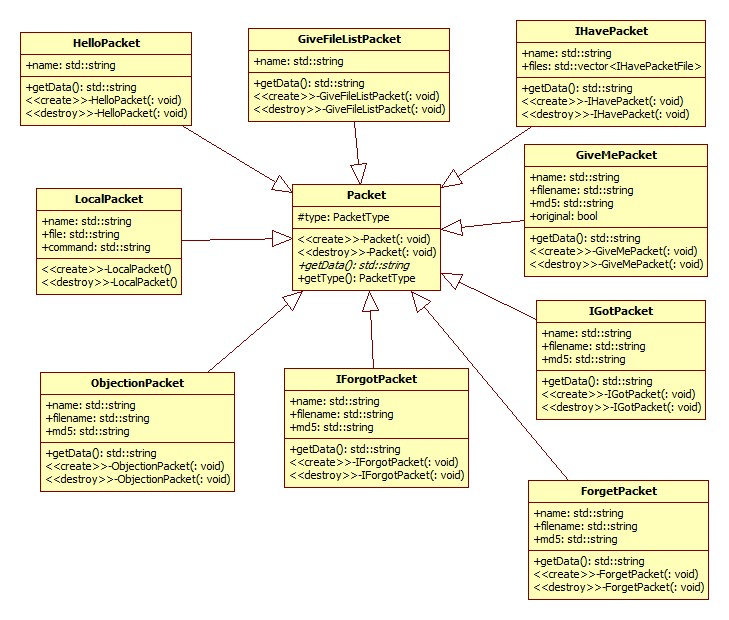
\includegraphics[width=\linewidth]{packet}
\section{Poprawność protokołu.}
\begin{itemize}
\item Nie jest możliwa sytuacja, gdy dwa węzły będą posiadać tą samą nazwę hosta. Sytuacja, gdy dołącza się taki, który próbuje uzyskać zajętą już nazwę jest opisana w punkcie protokołu, ciekawsza jest sytuacja, gdy dwa naraz taką samą nazwę spróbują zarezerwować. Jednak nie będzie tu problemu przez “symetrię”. Jako, że dwa naraz wyślą pakiety “Hello”, efekt będzie taki sam, jakby któryś z nich był już w sieci, tylko oba będą musiały zmienić nazwę. Typowy, równouprawniony kompromis.
\item Analogiczna sytuacja z plikami o tych samych nazwach nie jest
całkowicie niemożliwa, gdyż pliki definiowane są w naszym systemie poprzez
ich hash MD5. Takich hashy jest jednak ok. $2^{128}$, więc szansa,
że zdarzy się w sieci kolizja hashy plików jest pomijalnie mała.
\item Sytuacja, gdy ktoś próbuje pobrać plik, którego nikt z aktualnie aktywnych hostów nie posiada jest rozwiązana intuicyjnie - nie zostanie pobrany oraz użytkownik dowie się o błędzie.
\item Sytuacja, kiedy plik zostanie usunięty pod nieobecność kogoś
posiadającego kopię jest rozwiązana w następujący sposób -
przy następnym spotkaniu z kimkolwiek, kto kiedykolwiek posiadał ten plik
i stracił go z przyczyny wiadomości “Forget”  usunie go poprzez
powiadomienie.
\item Plik może być pobierany w kawałkach, a nawet posiada możliwość wznowienie pobierania! Wystarczy kiedy indziej pobrać plik, podając odpowiednie offsety i rozmiary kawałków brakujących!
\item Pliki zostaną usunięte w przypadku unieważnienia, nawet jeżeli utracą kontakt z hostem oryginalnym. Jednak klient będzie pamiętał hashe usuniętych plików i jeżeli okaże się, że pomimo braku kontaktu przez datę ważności plik nie został usunięty, będzie on pobrany przy najbliższej sposobności. Jest to rozwiązanie lepsze w sytuacji, gdy sieć jest duża bądź pliki są popularne (większość jest na dużej ilości hostów) bądź wszystkie hosty są aktywne. Gwarantuje to nie przechowywanie martwych plików więcej niż jest to konieczne płacąc za to możliwością usunięcia aktywnego pliku w skrajnych sytuacjach.
\end{itemize}

\section{Struktura}
Program będzie składał się z dwóch procesów. Pierwszy, proces serwera, będzie przez cały czas działać w tle, jest odpowiedzialny za zarządzanie zasobami oraz komunikację z innymi węzłami w sieci.
Drugi, proces klienta, będzie odpowiedzialny za komunikację pomiędzy użytkownikiem a serwerem. Komunikacja pomiędzy klientem a serwerem odbywać się będzie za pomocą socketów IPC. Sam klient będzie jednowątkowym programem wykonującym się na zasadzie przekazania polecenia użytkownika do serwera po wywołaniu, i następnie zakończenia działania po wypisaniu komunikatu zwrotnego.
Proces klienta będzie podzielony na kilka wątków, z których
\begin{itemize}
\item Jeden będzie odpowiedzialny za interakcje z użytkownikiem.
\item Jeden będzie przeznaczony na nasłuchiwanie broadcastów UDP od innych węzłów.
\item Pula węzłów będzie przeznaczona na połączenia TCP od/do innych węzłów.
\end{itemize}
Zaimplementowano klasy dostarzające narzędzi służących do realizacji funkcjonalności programu. \\
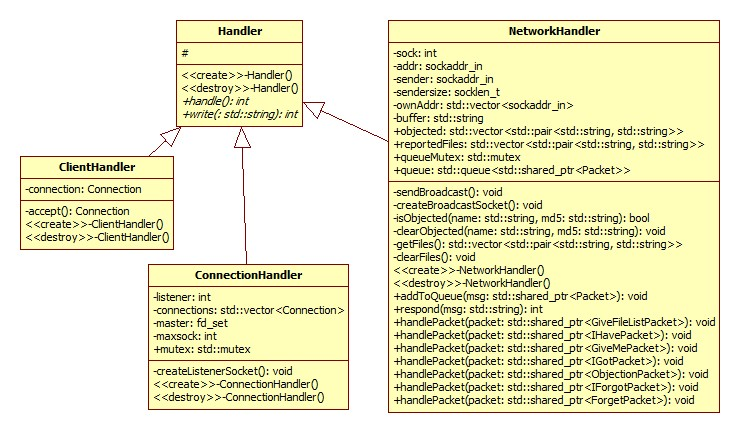
\includegraphics[width=\linewidth]{handler}
\textbf{ClientHandler} - realizuje funkcjonalność klienta. Nasłuchuje nadchodzące pakiety i reaguje zgodnie z przyjętym protokołem. \\
\textbf{NetworkHandler} - odpowiedzialny za komunikację sieciową. Umożliwia rozgłaszanie pakietów w sieci i w ospoweidni sposób reaguje na odebrane pakiety. \\
\textbf{ConnectionHandler} - obsługuje połączenia TCP. Umożliwia nawiązanie połączenia oraz odbiór i przesyłanie danych. \\


\section{ Zarys architektury i narzędzi.}
Projekt powstanie w języku C++, przy użyciu API gniazd BSD do komunikacji poprzez sieć, API gniazd IPC do komunikacji pomiędzy procesami. Dodatkowo w projekcie użyjemy bibliotek Boost oraz JSONCpp. W celu stworzenia dokumentacji skorzystamy z pakietu doxygen.




\end{document}